%ujednaciti opise signala u tablici
\documentclass[table,usenames,dvipsnames]{beamer}

\usepackage[english]{babel}
\usepackage[utf8]{inputenc}
\usepackage{listings}
\usepackage{datetime}
\usepackage{graphics}
\usepackage{fancybox}
\usepackage{color}
\usepackage[normalem]{ulem}
\usepackage{tikz}
\usepackage{verbatim}
\usetikzlibrary{shapes,arrows}
\usetheme{CambridgeUS}
\usecolortheme{seagull}
% Changing of bullet foreground color not possible if {itemize item}[ball]
\DefineNamedColor{named}{Purple}{cmyk}{0.52,0.97,0,0.55}
\setbeamertemplate{itemize item}[triangle]
\setbeamercolor{title}{fg=Purple}
\setbeamercolor{frametitle}{fg=Purple}
\setbeamercolor{itemize item}{fg=Purple}
\setbeamercolor{section number projected}{bg=Purple,fg=white}
\setbeamercolor{subsection number projected}{bg=Purple}

\renewcommand{\dateseparator}{.}
\newcommand{\todayiso}{\twodigit\day \dateseparator \twodigit\month \dateseparator \the\year}
\newcommand{\shell}[1]{\texttt{#1}}
\definecolor{LightGray}{gray}{0.9}

\title{Osnove korištenja operacijskog sustava Linux}
\subtitle{09. Procesi}
\author[Goran Cetušić]{Goran Cetušić\\{\small Nositelj: dr. sc. Stjepan Groš}}
\institute[FER]{Sveučilište u Zagrebu \\
				Fakultet elektrotehnike i računarstva}
				
\date{\todayiso}

\begin{document}
    %\beamerdefaultoverlayspecification{<+->}
{
\setbeamertemplate{headline}[] % still there but empty
\setbeamertemplate{footline}{}

\begin{frame}
\maketitle
\end{frame}
}

\begin{frame}
\frametitle{Sadržaj}
\tableofcontents
\end{frame}

\section{Pojam procesa}
\begin{frame}[t]
\frametitle{Pojam procesa (1)}
\begin{itemize}
  \item Program
  \begin{itemize}
    \item Datoteka s izvršnim kodom na disku računala
    \item Primjerice, \shell{/bin/bash} je program
  \end{itemize}
  \item Proces
  \begin{itemize}
    \item Program koji se izvršava na računalu
    \item Dakle, proces uključuje i niz dinamičkih podataka koji se mijenjaju 
          tijekom njegova izvršavanja a mogu se nalaziti pohranjeni na disku              ili u radnoj memoriji
  \end{itemize}
\end{itemize}
\end{frame}

\begin{frame}[t]
\frametitle{Pojam procesa (2)}
\begin{itemize}
  \item Svaki proces posjeduje jedinstveni identifikator
  \begin{itemize}
    \item PID – \emph{process identifier}
  \end{itemize}
  \item Proces koji je pokrenuo trenutni proces je njegov roditelj, svi 
        procesi pokrenuti od trenutnog procesa su njegova djeca
  \begin{itemize}
    \item PPID – parent PID
    \begin{itemize}
      \item Iznimka je proces za kojeg vrijedi PID=1 kojega je stvorila 
            jezgra operacijskog sustava tijekom inicijalizacije sustava
    \end{itemize}
  \end{itemize}
\end{itemize}
\end{frame}

\begin{frame}[t]
\frametitle{Unix procesi}
\begin{itemize}
  \item Pokretanje novog procesa ostvaruje se pozivanjem fork() funkcije unutar
        trenutnog programa
  \begin{itemize}
    \item fork() stvara kopiju procesa i vraća PID novonastalog procesa ili 0 
          ako je proces novonastali proces
  \end{itemize}
  \item Svaki roditelj odgovoran je počistiti za djetetom :)
  \begin{itemize}
    \item Roditelj čeka da dijete za vrši sa izvođenjem preko wait() sistemskog
          poziva
  \end{itemize}
\end{itemize}
\end{frame}

\section{Ispis procesa}
\begin{frame}[t]
\frametitle{Ispis procesa (1)}
\begin{itemize}
  \item Ispis procesa obavlja se s naredbom \shell{ps} 
  \begin{itemize}
    \item engl. \emph{processor status}
    \item ako se naredba pokrene bez argumenata i opcija ispisuje procese 
          vezane uz terminal na kojemu je pokrenuta
  \end{itemize}
  \item Omogućuje tri načina rada: Unix, BSD, GNU
  \item Zadatak:
  \begin{itemize}
    \item U man stranicama pogledati ispis svih procesa korištenjem UNIX i BSD 
          načina
  \end{itemize}
\end{itemize}
\end{frame}

\begin{frame}[t]
\frametitle{Ispis procesa (2)}
\begin{itemize}
  \item Ispis naredbe \shell{ps} sadrži sljedeće kolone
  \begin{tabular}{l l}
    PID   & ID procesa \\
    TTY   & TTY za koji je proces vezan \\
    TIME  & Ukupno vrijeme izvršavanja  \\
    CMD   & Naredba bez argumenata
  \end{tabular}
\end{itemize}
\end{frame}

\begin{frame}[t]
\frametitle{Ispis procesa (3)}
\begin{itemize}
  \item Dodatne informacije o procesima ispisuju se korištenjem opcije 
        \shell{-f}
  \begin{tabular}{l l}
    UID   & Vlasnik procesa \\
    PPID  &   Roditelj procesa \\
    CMD   &   Naredba s argumentima
  \end{tabular}
\end{itemize}
\end{frame}

\begin{frame}[t]
\frametitle{Ispis procesa (4)}
\begin{itemize}
  \item Korisne opcije \shell{ps} naredbe
  \begin{tabular}{l l}
    \shell{-e}        & ispis svih procesa na sustavu \\
    \shell{-f}        & dodatne informacije o procesima \\
    \shell{-o}        & zadavanje ispisa željenih informacija \\
    \shell{-{}-sort}  & sortiranje ispisa (po PID ako nije navedeno)
  \end{tabular} 
\end{itemize}
\end{frame}

\begin{frame}[t]
\frametitle{Ispis procesa (5)}
\begin{itemize}
  \item Primjeri
  \begin{itemize}
    \item ispis trenutnih procesa sa definiranim prikazom atributa
    \item[] \shell{ps -eo pid, ppid,user,args,nice --sort user}
    \item detaljan ispis SVIH procesa, uključujući dretve
    \item[] \shell{ps -eLf}
  \end{itemize}
\end{itemize}
\end{frame}

\begin{frame}[t]
\frametitle{Ispis procesa (6)}
\begin{itemize}
  \item S argumentom \shell{u} dobijamo ispis resursa što ih troše procesi
  \begin{itemize}
    \item Kolone specifične za ovaj ispis
    \begin{tabular}{l l}
      \%CPU   & Količina ``potrošnje'' procesora  \\
      \%MEM   & Količina zauzete radne memorije \\ 
      VSZ     & Virtualna veličina memorije \\
      STAT    & Stanje procesa u trenutku izvršavanja naredbe \\
      START   & Vrijeme kada je naredba pokrenuta
    \end{tabular}
  \end{itemize}
\end{itemize}
\end{frame}

\begin{frame}[t]
\frametitle{Stanja procesa}
\begin{itemize}
  \item Moguće vrijednosti statusa procesa
    \begin{tabular}{l l}
      \textbf{R}  & aktivni (engl. \emph{running}) proces \\
      \textbf{S}  & spavajući (engl. \emph{sleeping}) proces (20 sekundi ili 
                    manje) \\
      \textbf{I}  & besposlen (engl. \emph{idle}) proces (više od 20 sekundi) \\
      \textbf{T}  & zaustavljen (engl. \emph{stopped}) proces \\
      \textbf{Z}  & zombi proces (proces koji je završio, ali zauzima zapis u 
                    tablici \\ & procesa)
    \end{tabular}
\end{itemize}
\end{frame}

\begin{frame}[t]
\frametitle{Dodatne naredbe za ispis (1)}
\begin{itemize}
  \item \shell{pgrep} pretražuje procese na temelju imena i drugih atributa
  \item Zadatak
  \begin{itemize}
    \item Pretražite procese korisnika root
  \end{itemize}
  \item \shell{pstree} ispisuje stablo svih procesa na sustavu
  \item Zadatak
  \begin{itemize}
    \item Provjerite odnose procesa pomoću naredbe \shell{pstree}
  \end{itemize}
\end{itemize}
\end{frame}

\begin{frame}[t]
\frametitle{Dodatne naredbe za ispis (2)}
\begin{itemize}
  \item Naredba \shell{ps} ispise trenutno stanje svih procesa (snapshot)
  \begin{itemize}
    \item Naredba \shell{top} omogućuje konstantan ispis
  \end{itemize}
  \item Podrazumijevane vrijednosti naredbe \shell{top}
  \begin{itemize} 
    \item Osvježavanje se obavlja svake 3 sekunde
    \item Tipka s i upisivanje broja mijenja tu vrijednost
    \item Procesi su poredani po korištenju procesora
    \item S tipkom M poredak se vrši po potrošnji memorije, tipkom P po 
          korištenju procesora
  \end{itemize}
\end{itemize}
\end{frame}

\section{Slanje signala}
\begin{frame}[t]
\frametitle{Slanje signala (1)}
\begin{itemize}
  \item Signal je programski prekid (engl. \emph{interrupt})
  \item Kada primi signal, proces obavlja neku akciju ili obradu, ili jezgra 
        operacijskog sustava obavlja akciju
  \begin{itemize}
    \item Po završetku obrade proces nastavlja s normalnim izvršavanjem
  \end{itemize}
  \item Svaki signal ima svoj broj i skraćeno ime
  \begin{itemize}
    \item  Ime signala služi korisnicima, a brojevi jezgri
  \end{itemize}
\end{itemize}
\end{frame}

\begin{frame}[t]
\frametitle{Slanje signala (2)}
\begin{itemize}
  \item Slanje signala iz komandne linije obavlja se naredbom \shell{kill}
  \begin{itemize}
    \item Tipke Ctrl+C i slične također šalju signale procesima!
  \end{itemize}
  \item Ako je zaustavljen roditelj i dijete će biti zaustavljeno
  \begin{itemize}
    \item Svaki proces kao svog pretka ima init proces
  \end{itemize}
\end{itemize}
\end{frame}

\begin{frame}[t]
\frametitle{Slanje signala (3)}
\begin{itemize}
  \item Sintaksa
  \begin{itemize}
    \item[] \shell{kill [-<broj signala>] <PID>}
  \end{itemize}
  \item Popis svih raspoloživih signala se može dobiti opcijom \shell{-l}
  \begin{table}[h]
  \rowcolors{1}{White}{LightGray}
  \begin{tabular}{l l l}
    \rowcolor{BlueViolet!20}Broj  & Ime & Značenje  \\
    1   & SIGHUP  & Završiti s radom (engl. \emph{hang up}) \\
    2   & SIGINT  & Prekidanje (engl. \emph{interrupt}) \\
    9   & SIGKILL & Kill (ne može biti ignoriran) \\
    15  & SIGTERM & Programska terminacija (podrazumijevani signal)
  \end{tabular}
  \end{table}
\end{itemize}
\end{frame} 

\begin{frame}[t]
\frametitle{Slanje signala (4)}
\begin{itemize}
  \item Naredba \shell{killall} služi za slanje signala na temelju imena, za 
        razliku od \shell{kill} naredbe (PID)
  \item Zadatak:
  \begin{itemize}
    \item Terminirajte proces s PID = 1
    \begin{itemize}
      \item  Što se dogodilo?
    \end{itemize}
    \item Otvorite dva terminala. Terminirajte ljusku onog drugog.
    \begin{itemize}
      \item Što se dogodilo?
      \item Pošaljite signal broj 9 (KILL) ljusci drugog terminala.
      \item Što se sada desilo?
    \end{itemize}
  \end{itemize}
\end{itemize}
\end{frame}

\begin{frame}[t]
\frametitle{Mijenjanje prioriteta procesa}
\begin{itemize}
  \item Kod rezerviranja CPU vremena neki procesi neki procesi imaju veći 
        prioritet
  \begin{itemize}
    \item Ali većina korisničkih programa ima isti priotitet
  \end{itemize}
  \item Naredbom \shell{nice} procesi se pokreću sa višim ili nižim prioritetom
  \begin{itemize}
    \item \shell{renice} mijenja prioritet postojećeg procesa ili grupe procesa
  \end{itemize}
  \item Zadatak:
  \begin{itemize}
    \item Odaberite proces i promijenite mu prioritet!
  \end{itemize}
\end{itemize}
\end{frame}

\section{Odvijanje procesa u pozadini}
\begin{frame}[t]
\frametitle{Poslovi}
\begin{itemize}
  \item Ljuske prepoznaju koncept poslova (engl. \emph{jobs})
  \begin{itemize}
    \item Kod pokretanja procesa iz terminala ljuska proces stavi u prednji 
          plan (engl. \emph{foreground})
  \end{itemize}
  \item Proces je moguće prebaciti u pozadinu i u prednji plan ili zaustaviti
  \begin{itemize}
    \item[] Ctrl+Z
    \item[] \shell{bg}
    \item[] \shell{fg}
    \item[] \shell{jobs}
  \end{itemize}
\end{itemize}
\end{frame}

\begin{frame}[t]
\frametitle{Naredba \shell{bg}}
\begin{itemize}
  \item Ako se proces nastavlja bez ikakvog ispisa na ekran i bez ikakvih 
        zahtjeva za unosom, koristimo naredbu \shell{bg} da ga stavimo u 
        pozadinu, gdje će se odvijati dok se ne završi
  \begin{itemize}
    \item naredbu \shell{bg} možemo koristiti tek nakon suspendiranja procesa 
          naredbom Ctrl+Z
    \item Posljedica Ctrl+Z je slanje signala SIGSTOP procesu
  \end{itemize}
  \item Terminiranje ljuske terminira njezine procese
\end{itemize}
\end{frame}

\begin{frame}[t]
\frametitle{Naredba \shell{jobs}}
\begin{itemize}
  \item Naredba \shell{jobs} prikazuje nam procese koji se izvršavaju u pozadini
  \begin{itemize}
    \item Procesi imaju identifikator koji \textbf{nema veze} s PID-om
  \end{itemize}
  \item Taj identifikator može se koristiti kod naredbe \shell{bg} i sličnih
\end{itemize}
\end{frame}

\begin{frame}[t]
\frametitle{Naredba \shell{fg}}
\begin{itemize}
  \item Kada je proces zaustavljen ili se izvršava u pozadini, 
        može se ponovno staviti u aktivan način rada naredbom \shell{fg} 
        (engl. \emph{foreground})
  \begin{itemize}
    \item puno naredbi koje rade s procesima prihvaćaju identifikator/oznaku 
          posla (jobID) kao argument pa tako i naredba \shell{fg}
  \end{itemize}
  \item Ako identifikator nije naveden, podrazumijeva se zadnji proces s kojim 
        je nešto napravljeno
\end{itemize}
\end{frame}

\begin{frame}[t]
\frametitle{Korištenje \shell{bg,jobs} i \shell{fg} (1)}
\begin{itemize}
  \item Pokrenuti editor \shell{vi} te ga zaustaviti sa 
        \shell{\textasciicircum{}Z}
  \item Pogledati naredbom \shell{jobs} aktivne poslove
  \item Pokrenuti još jedan proces programa \shell{vi} te ga također zaustaviti
        sa \shell{\textasciicircum{}Z}
  \item Ponovo upotrijebiti naredbu \shell{jobs} i pogledati aktivne poslove
  \begin{itemize}
    \item S oznakom + označen je zadnji proces s kojim je nešto manipulirano, 
          a oznakom – označen je predzadnji
  \end{itemize}
\end{itemize}
\end{frame}

\begin{frame}[t]
\frametitle{Korištenje \shell{bg,jobs} i \shell{fg} (2)}
\begin{itemize}
  \item Primjetite kako su svi procesi u stanju Stopped
  \begin{itemize}
    \item S naredbom \shell{bg} prebacite proces s JID-om 1 u pozadinu
    \item Što se desilo? Nastavlja li se proces izvršavati u pozadini?
  \end{itemize}
  \item Naredba \shell{kill} prihvaća i JID, ali ga je potrebno označiti s \%
  \begin{itemize}
    \item Pošaljite signal TERM vi editoru s JID-om 1
    \item Što se desilo? Stavite posao 1 u prednji plan (\shell{fg 1})
  \end{itemize}
\end{itemize}
\end{frame}

\begin{frame}[t]
\frametitle{Operator \&}
\begin{itemize}
  \item Nije nužno pokretati program pa ga zaustavljati sa 
        \shell{\textasciicircum{}Z}
  \begin{itemize}
    \item Možemo koristiti operator \& kod pokretanja programa
    \item Ako program zahtijeva unos ili ispis, zaustavlja se
    \begin{itemize}
      \item to ne ovisi o tome kako je program pokrenut
    \end{itemize}
  \end{itemize}
  \item Da bi se program odmah pokrenuo u pozadini, jednostavno napišite \& na 
        kraju komandne linije
\end{itemize}
\end{frame}

\begin{frame}[t]
\frametitle{Procesi, grupe procesa i sjednice (1)}
\begin{itemize}
  \item Pokrenuti proces vezan je na terminal
  \begin{itemize}
    \item Terminiranjem ljuske prekinut je i proces
  \end{itemize}
  \item Svaki proces dio je grupe procesa
  \begin{itemize}
    \item Grupa procesa je obuhvaća isto što i posao
    \item Neke ljuske ne podržavaju poslove
  \end{itemize}
  \item Svaka grupa procesa dio je sjednice
  \begin{itemize}
    \item Ovakvo grupiranje omogućuje slanje signala svim željenim procesima 
          istovremeno
  \end{itemize}
\end{itemize}
\end{frame}

\begin{frame}[t]
\frametitle{Procesi, grupe procesa i sjednice (2)}
\begin{itemize}
  \item Primjer
  \begin{itemize}
    \item[] \shell{\$ cat}
    \item[] \shell{hello}
    \item[] \shell{hello}
    \item[] \shell{\textasciicircum{}Z}
    \item[] \shell{[1]+ Stopped}
    \item[] \shell{\$ ls | sort}
  \end{itemize}
  \item Identifikator grupe procesa (PGID) jednak je identifikatoru prvog 
        procesu grupe 
  \item Svi procesi povezani cjevovodom su dio iste grupe
  \item Svi procesi unutar ljuske su dio iste sjednice
\end{itemize}
\end{frame}

\begin{frame}[t]
\frametitle{Procesi, grupe procesa i sjednice (3)}
\begin{itemize}
  \item Slika otprilike pokazuje stanje prethodnog primjera
  \begin{itemize}
    \item Primijetite kako je moguće ne imati TTY postavljen
  \end{itemize}
\end{itemize}
    \flushleft
    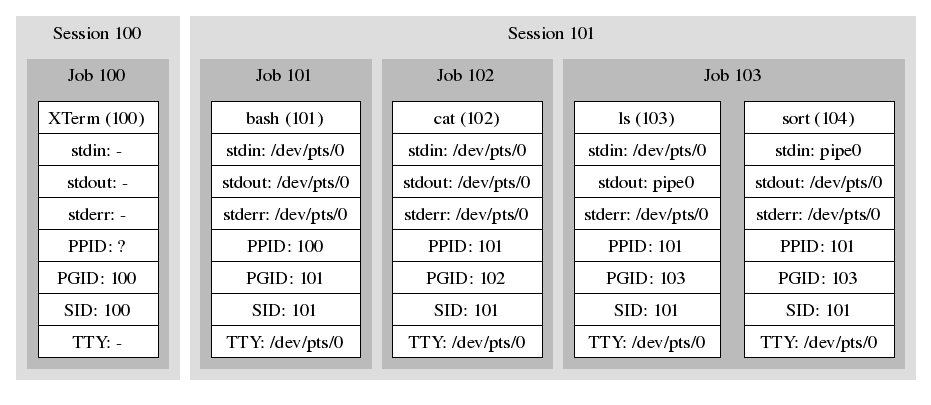
\includegraphics[scale=0.35]{process.png}
\end{frame}

\begin{frame}[t]
\frametitle{Literatura}
\begin{itemize}
  \item \url{http://www.linux.com/archive/feature/125977}
  \item \url{http://www.linux-tutorial.info/modules.php?name=MContent&pageid=84}
  \item \url{http://www.linuxhq.com/guides/SAG/x1826.html}
  \item \url{http://www.win.tue.nl/~aeb/linux/lk/lk-10.html}
  \item \url{http://www.linusakesson.net/programming/tty/index.php}
\end{itemize}
\end{frame}







\end{document}
